% Basic stuff
\documentclass[a4paper,10pt]{article}
\usepackage[swissgerman]{babel}

% 3 column landscape layout with fewer margins
\usepackage[landscape, left=0.5cm, top=0.75cm, right=0.75cm, bottom=1cm, footskip=15pt]{geometry}
\usepackage{flowfram}
\ffvadjustfalse
\setlength{\columnsep}{0.75cm}
\Ncolumn{3}

% Remove paragraph indentation
\setlength{\parindent}{0pt}

% For defining line spacing
\usepackage{setspace}

\usepackage{multicol}

% For inserting figures
\usepackage{wrapfig}

% For enumeration with letters
\usepackage[shortlabels]{enumitem}

% Define nice looking boxes
\usepackage[many]{tcolorbox}

% Base style for boxes
\tcbset{
  base/.style={
    boxrule=0.2mm,
    left=1.75mm,
    arc=0mm,
    fonttitle=\bfseries,
    colbacktitle=black!10!white,
    coltitle=black,
    toptitle=0.75mm,
    bottomtitle=0.25mm,
    title={#1}
  }
}
\definecolor{backcol}{RGB}{240,240,240}
\definecolor{brandblue}{rgb}{0, 0, 0}
\newtcolorbox{mainbox}[1]{
  colframe=brandblue,
  colback=backcol,
  base={#1}
}

\definecolor{backcol2}{RGB}{255,255,255}
\definecolor{brandblue2}{rgb}{0, 0, 0}
\newtcolorbox{subbox}[1]{
  colframe=black!20!white,
  colframe=brandblue2,
  colback=backcol2,
  base={#1}
}

\newtcolorbox{subbox_noTitle}[1][]{
  colframe=black!20!white,
  colframe=brandblue2,
  colback=backcol2,
  base={#1},
  title=#1
}


% Mathematical typesetting & symbols
\usepackage{amsthm, mathtools, amssymb, amsmath}
\usepackage{marvosym, wasysym}
\allowdisplaybreaks

% Tables
\usepackage{tabularx, multirow}
\usepackage{makecell}
\usepackage{booktabs}
\renewcommand*{\arraystretch}{2}

% Make enumerations more compact
\newenvironment{myitemize}
{\vspace{-0.25cm}\begin{itemize}}
{\end{itemize}}
\setlist[itemize]{leftmargin=10pt, itemsep=0.5pt}

\setlist[enumerate]{leftmargin=10pt, itemsep=0.75pt}

% To include sketches & PDFs
\usepackage{graphicx}

% For hyperlinks
\usepackage{hyperref}
\hypersetup{
  colorlinks=true
}

% Metadata (fixing the inline title format)
\title{\textbf{Machine Learning in Finance and Insurance}}
\author{}
\date{}

% Reduces space above and below the title
\usepackage{titling}
\setlength{\droptitle}{-1.5cm}
% \posttitle{\par\vspace{-0.5cm}}

% Math helper stuff
\def\limn{\lim_{n\to \infty}}
\def\limxo{\lim_{x\to 0}}
\def\limxi{\lim_{x\to\infty}}
\def\limxn{\lim_{x\to-\infty}}
\def\sumk{\sum_{k=1}^\infty}
\def\sumn{\sum_{n=0}^\infty}
\def\R{\mathbb{R}}
\def\dx{\text{ d}x}
\def\P{\mathbb{P}}
\def\F{\mathcal{F}}
% \def\E{\mathcal{E}}
\DeclareMathOperator{\E}{\mathbb{E}}
\DeclareMathOperator{\Var}{Var}

% Use small subtitles
\newcommand{\subtitle}[1]{\begin{normalsize}\vspace{0.25cm}\textbf{#1} \end{normalsize}}


\begin{document}

% Add title
\maketitle

% Reduce space
\vspace{-3cm}


\begin{center}
    \textbf{Ramon Kaspar, ETH Zürich (Fall 2024)}
\end{center}

\begin{small}

\section{Basic Notions of Statistical Learn.}

\begin{subbox}{Expected Loss (Expected Risk)}
\[
\E[\ell(f(X), Y)] = \int_{\mathcal{X} \times \mathcal{Y}} \ell(f(x), y) \rho(dx, dy).
\]
For a measurable \textit{loss function} \(\ell : \mathcal{Y} \times \mathcal{Y} \to \R^+\)
\end{subbox}
Goal: Find \(f\) that minimizes \(\E[\ell(f(X), Y)]\).

\begin{subbox}{Empirical Loss (Empirical Risk)}
    With training data $(X_i, Y_i)_{i=1}^m$: 
    \[
        \E[\ell(f(X), Y)] \approx \frac{1}{m} \sum_{i=1}^m \ell(f(X_i), Y_i).
    \]
\end{subbox}
\(\Rightarrow\) Empirical loss minimizer depends on hypothesis class \(\mathcal{H}\) and loss function \(\ell\). For square loss and constant functions, the minimizer is \(\bar{Y} = \frac{1}{m} \sum_{i=1}^{m} Y_i\). There's a \textit{Bias-Variance Tradeoff}; the best balance depends on the unknown distribution of \(Y\).

\subtitle{Pred. Prob.:} 
Find meas. func. \(f: \mathcal{X} \rightarrow \mathcal{Y}\), s.t. \(f(X) \approx Y\).

\subtitle{Hypothesis Class:} 
A \textit{hypothesis class} is a family \(\mathcal{H}\) of measurable functions \(f : \mathcal{X} \to \mathcal{Y}\), e.g. all affine functions.

\subtitle{Model Estimation:}
Find a numerical solution \(\hat{f}_m\) to:
\begin{footnotesize}  
\[
\min_{f \in \mathcal{H}} \frac{1}{m} \sum_{i=1}^m \ell(f(X_i), Y_i)
\]
\end{footnotesize}
\begin{myitemize}
    \item \textbf{Deterministic algorithm:} \(\hat{f}_m(\cdot) = \hat{\varphi}\left( \cdot , (X_i, Y_i)_{i=1}^m \right)\)
    \item \textbf{Stochastic algorithm} (e.g., random initialization): \(\hat{f}_m(\cdot) = \hat{\varphi}\left( \cdot , (X_i, Y_i)_{i=1}^m, V \right)\), where \(V\) indep. of \((X, Y)\) \& random.
\end{myitemize}
Define the average model \(\hat{f}_m^{\text{avg}}(x) := \E[\hat{f}_m(x)]\).

\subtitle{Relationships between $X$ and $Y$:}
\vspace{0.2cm}
\begin{myitemize}
    \item \textit{Deterministic dependence:} $Y = g(X)$
    \item \textit{Homoscedastic additive noise:} $Y = g(X) + \epsilon$, for $\epsilon$ independent of $X$ with $\E[\epsilon] = 0$
    \item \textit{Heteroscedastic additive noise:} $Y = g(X) + h(X)\epsilon$, for $\epsilon$ independent of $X$ with $\E[\epsilon] = 0$
    \item \textit{Non-additive noise:} $Y = g(X, \epsilon)$, for $\epsilon$ independent of $X$
    \item \textit{Model-free:} the form of the underlying model is not known, only iid observations $(X_i, Y_i)_{i=1}^m$ are available
\end{myitemize}


\subtitle{Regression Function:}
\(\bar{f}(x)\) minimizes \(w \mapsto \int_{\mathcal{Y}} \ell(w, y) \rho_{Y|X}(dy | x)\) and is called the \textit{regression function}. \(\E[\ell(\bar{f}(X), Y)]\) is the \textit{irreducible error}.

\textbf{\textit{Square Loss}} \(\bar{f}(X) = \E[Y | X]\), \(\E[\ell(\bar{f}(X), Y)] = \Var(Y) - \Var(\E[Y | X])\) 

\textbf{\textit{Pinball Loss}}
\( \ell_{\alpha}(u) = \left( \alpha - 1_{\{u < 0\}} \right) u \text{ for } u \in \R \), \(\bar{f}(X) = q_\alpha\) and \(\E[\ell(\bar{f}(X), Y)] = \E \left[ \ell_\alpha( Y - q_\alpha(X) ) \right ])\) 

\begin{subbox}{Bias-Variance Decomposition of Square Loss}
\begin{align}
E\left[ (\hat{f}_m(X) - Y)^2 \right] = 
\underbrace{ \E \left[ \left( \hat{f}_m^{\text{avg}}(X) - \bar{f}(X) \right)^2 \right]}_{\text{Bias}^2} + \notag  \\
 \underbrace{E\left[ \left( \hat{f}_m(X) - \hat{f}_m^{\text{avg}}(X) \right)^2 \right] }_{\text{Variance}} \notag 
 + \underbrace{E\left[ \left( \bar{f}(X) - Y \right)^2 \right]}_{\text{Irreducible Error}}. \notag
\end{align}
\end{subbox}

% Insert Image Bia-Variance Tradeoff
\begin{wrapfigure}{r}{0.5\columnwidth}
    \centering
    \vspace{-20pt}
    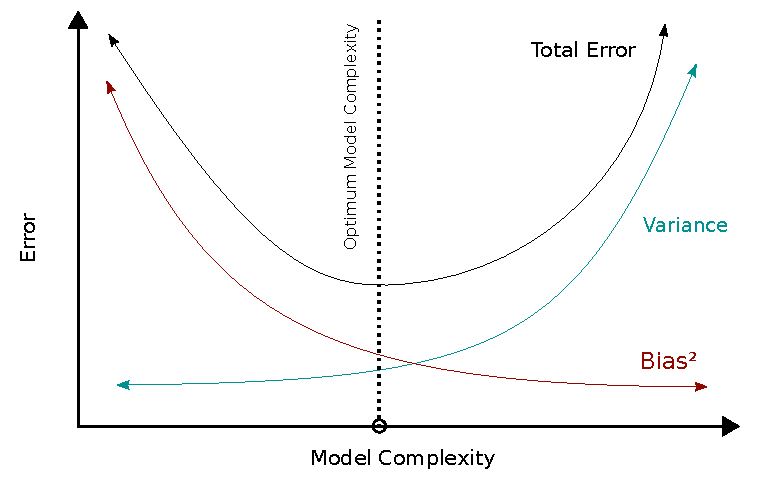
\includegraphics[width=0.45\columnwidth]{figures/Bias_and_variance_contributing_to_total_error.pdf}
    \vspace{-30pt}
\end{wrapfigure}

\textbf{Bias}: Error from erroneous assumptions (underfitting). \\
\textbf{Variance}: Error from sensitivity to data fluctuations (overfitting). \\
\textbf{Trade-off}: Increase model complexity $\Rightarrow$ lower bias, higher var

\begin{subbox}{$R^2$ \quad (goodness of in-sample fit)}
    Let $(X_i, Y_i)_{i=1}^m$ be the training data, and $(X_i, Y_i)_{i=m+1}^{m+n}$ the test data.
    Let $\hat{f}_m: \mathcal{X} \to \mathcal{Y}$ be a prediction function trained on training data:

    \[R^2 = 1 - \frac{SSR}{SST}\]

    $\text{SSR} = \sum_{i=1}^{m} \left( Y_i - \hat{f}_m(X_i) \right)^2$, $\text{SST} = \sum_{i=1}^{m} \left( Y_i - \overline{Y}_{\text{train}} \right)^2$ for $\quad \overline{Y}_{\text{train}} = \frac{1}{m} \sum_{i=1}^{m} Y_i$. \textit{The higher the better}.
\end{subbox}

Similarly, define out-of-sample \(R^2_{\text{os}}\) using test data; it measures \textbf{prediction power}.

\begin{subbox}{Approximation Error}
    $$\inf_{f \in \mathcal{H}} \mathbb{E} \, \ell(f(X), Y) - \mathbb{E} \, \ell(\overline{f}(X), Y) \geq 0$$
\end{subbox}
Approximation error occurs if $\mathcal{H}$ is not flexible enough to approximate $\bar{f}$ well. Is decreasing if $\mathcal{H}$ is increasing. Is $0$ if $\bar{f} \in \mathcal{H}$. 

If the empirical loss min. problem $\min_{f \in \mathcal{H}} \frac{1}{m} \sum_{i=1}^{m} \ell(f(X_i), Y_i)$ has a solution, we call it $\hat{f}_m^{\mathcal{H}} \in \mathcal{H}$.

\begin{subbox}{Sampling Error}
\begin{footnotesize}
    $$\E \left[ \ell \left( \hat{f}_m^{\mathcal{H}}(X), Y \right) \middle| \hat{f}_m^{\mathcal{H}} \right] 
- \inf_{f \in \mathcal{H}} \E [\ell(f(X), Y)] = $$
$$
\int_{\mathcal{X} \times \mathcal{Y}} \ell \left( \hat{f}_m^{\mathcal{H}}(x), y \right) \rho(dx, dy) 
- \inf_{f \in \mathcal{H}} \int_{\mathcal{X} \times \mathcal{Y}} \ell(f(x), y) \rho(dx, dy) \geq 0$$
\end{footnotesize}
\end{subbox}

Results from minimizing the empirical loss instead of the expected loss. Tends to decrease if the sample size $m$ is increasing.

\begin{subbox}{Direct Optimization Error}
Let $\hat{f}_m(\cdot) = \hat{\varphi}(\cdot, (X_i, Y_i)_{i=1}^{m}, V)
$:
    $$\frac{1}{m} \sum_{i=1}^{m} \ell \left( \hat{f}_m(X_i), Y_i \right) 
- \inf_{f \in \mathcal{H}} \frac{1}{m} \sum_{i=1}^{m} \ell \left( f(X_i), Y_i \right) \geq 0
$$
\end{subbox}
For classical methods (e.g., lin. reg.), assume \(\hat{f}_m \approx \hat{f}_m^{\mathcal{H}}\). For complex ML methods (boosted trees, NNs), typically \(\hat{f}_m \not\approx \hat{f}_m^{\mathcal{H}}\).

\begin{subbox}{Generalization Error}
\begin{footnotesize}
\[
\E\left[\ell(\hat{f}_m(X), Y) \mid \hat{f}_m\right]
= \E[\ell(\bar{f}(X), Y)] \quad \textit{(irreducible error)}
\]
\[
+ \inf_{f \in \mathcal{H}} \E[\ell(f(X), Y)] - \E[\ell(\bar{f}(X), Y)] \quad \textit{(approximation error)}
\]
\[
+ \E \left[\ell\left(\hat{f}_m^{\mathcal{H}}(X), Y\right) \mid \hat{f}_m^{\mathcal{H}}\right] - \inf_{f \in \mathcal{H}} \E[\ell(f(X), Y)] \quad \textit{(sampling error)}
\]
\[
+ \E \left[\ell\left(\hat{f}_m(X), Y\right) \mid \hat{f}_m\right] - \E \left[\ell\left(\hat{f}_m^{\mathcal{H}}(X), Y\right) \mid \hat{f}_m^{\mathcal{H}}\right] \textit{(ind. opt. error)}
\]
\end{footnotesize}
\end{subbox}
For fixed \(m \in \mathbb{N}\) and increasing \(\mathcal{H}\): approx. error decreases, sampling error increases (variance of \(\hat{f}_m^{\mathcal{H}}\) grows). There's a tradeoff between them (like bias-variance). For small data, \(\mathcal{H}\) should be simple; for large data, it can be complex.

\begin{subbox}{ Training Error and Test Error}
\begin{footnotesize}
$$E_{\text{tr}} = \frac{1}{m} \sum_{i=1}^{m} \ell\left(\hat{f}_m(X_i), Y_i\right), \ \ E_{\text{te}} = \frac{1}{m} \sum_{i=m+1}^{m+n} \ell\left(\hat{f}_m(X_i), Y_i\right)$$
\end{footnotesize}
\end{subbox}

If $E_{\text{tr}} \ll E_{\text{te}}$, the data most likely was overfitted. \\
\textbf{Sample Variance:} $\sigma_{\text{te}}^2 = \frac{1}{n-1} \sum_{i=m+1}^{m+n} \left( \ell\left(\hat{f}_m(X_i), Y_i\right) - E_{\text{te}} \right)^2$

\section{Linear Regression}

Linear regression models the relationship between predictors and response:
\(
y = \beta_0 + \beta_1 X_1 + \dots + \beta_d X_d + \epsilon, \quad \epsilon \sim N(0, \sigma^2)
\)
In matrix form:
\[
y = A\beta + \epsilon
\]
where \( A \) is the design matrix, \( \beta \) the coefficient vector.

\begin{subbox}{Normal Equation}
If $A^TA$ regular (or equivalently columns of $A$ lin. indep.):
\[
\hat{\beta} = \min_{b \in \mathbb{R}^{d+1}} \|A b - y\|_2^2
 = (A^\top A)^{-1} A^\top y
\]
\end{subbox}
$\Rightarrow \hat{\beta} = (A^T A)^{-1} A^T (A \beta + \epsilon) \sim \mathcal{N}_{d+1} \left( \beta, \sigma^2 (A^T A)^{-1} \right)$

If columns of \( A \) are linearly dependent, \( A^\top A \) is singular, and the normal equation has infinitely many solutions. The \textbf{pseudoinverse} solution \(\hat{\beta} = (A^\top A)^{\dagger} A^\top y\) minimizes \( \| b \|_2 \). Here, \((A^\top A)^{\dagger} = V \Lambda^{\dagger} V^\top\), with \(\Lambda^{\dagger}\) diagonal entries \(1_{\{\lambda_j > 0\}} \lambda_j^{-1}\).


\subtitle{Singular Value Decomposition (SVD)}

Matrix \( A \in \R^{m \times l}\), rank $r \leq \min(m,l)$, can be decomposed as:
\[
A = U \Sigma V^\top 
\]

\begin{myitemize}
    \item $U \in \R^{m \times m}$ and $V\in \R^{l \times l}$ orthogonal, $\Sigma^\dagger \in \R^{l \times m}$ diagonal
    \item $\lambda_1 \geq ... \geq \lambda_r$ are the positive eigenvalues of $A^\top A$ and $\Sigma = \text{diag}(\sqrt{\lambda_1}, ..., \sqrt{\lambda_r}, 0, ...) \in \R^{m \times l}$
    \item \textbf{Pseudoinverse} $A^\dagger = V \Sigma^\dagger U^\top$; for any $y \in \mathbb{R}^m, \hat{\beta} = A^{\dagger} y \in \mathbb{R}^n$ minimizes $b \mapsto \|A b - y\|_2$ with minimal $\|\cdot\|_2$-norm.
    \item \textbf{Regularization:} Truncate small \(\sigma_i\) (set \(\sigma_i = 0\) if \(\sigma_i < c\)); then \(\hat{\beta}_c = A_c^\dagger y \sim \mathcal{N}_l \left( Q_k \beta, \sigma^2 V \Lambda_c^{-1} V^T \right)\) balances bias and variance: increasing \( c \) increases bias and decreases variance.
\end{myitemize}

\begin{subbox}{Ridge Regression}
    $$\hat{\beta}_\lambda = \min_{b \in \mathbb{R}^{d+1}} \left( \|A b - y\|_2^2 + \lambda \|b\|_2^2 \right) = (A^\top A + \lambda I_l)^{-1} A^\top Y$$
\end{subbox}

\begin{footnotesize}
$\hat{\beta}_\lambda =  \sum_{i=1}^{r} \frac{\sigma_i}{\sigma_i^2 + \lambda} v_i u_i^T y \sim \mathcal{N}_l \left( \sum_{i=1}^{r} \frac{\lambda_i}{\lambda_i + \lambda} v_i v_i^T \beta, \sigma^2 \sum_{i=1}^{r} \frac{\lambda_i}{(\lambda_i + \lambda)^2} v_i v_i^T \right)$
\end{footnotesize}
\textit{Increasing \( \lambda \) increases bias and decreases variance}. 

\begin{subbox}{LASSO Regression}
\[
\hat{\beta}_\lambda = \min_{b \in \mathbb{R}^{d+1}} \left( \|A b - y\|_2^2 + \lambda \| \beta \|_1 \right)
\]
\end{subbox}
$\Rightarrow$ No closed-form solution, LASSO-Regr. encourages \textbf{sparsity}.

\subtitle{Cross-Validation}

Technique to estimate model's predictive performance and tune hyperparameters.
\begin{subbox_noTitle}
Divide data into \( K \) folds:
\begin{itemize}
    \item Train on \( K-1 \) folds.
    \item Validate on the remaining fold.
    \item Repeat \( K \) times; average validation error.
\end{itemize}
\end{subbox_noTitle}

\subtitle{Standardized Linear Regression} 
\[
\tilde{x}_i = \frac{x_i - \bar{x}}{s_x}, \quad  \tilde{y}_i = \frac{y_i - \bar{y}}{s_y}
\]
with mean \( \bar{x}_j \) and $s_j^2 = \frac{1}{m} \sum_{i=1}^{m} \left( x_{ij} - \bar{x}_j \right)^2$. The prediction $\hat{y}$ for a new datapoint $x=(x_1,...,x_d)$ is $\hat{y} = s_y \sum_{j=1}^{d} \frac{x_j - \bar{x}_j}{s_j} \hat{\beta}_j + \bar{y}$

\section{Gradient Descent}

A function $ h : \mathbb{R}^d \to \mathbb{R}$ is said to be \textbf{\textit{convex}} if $
h(\lambda x + (1 - \lambda) y) \leq \lambda h(x) + (1 - \lambda) h(y)$, for all $ x, y \in \mathbb{R}^d \text{ and } \lambda \in (0,1)$.

\textbf{Setup}: Given a convex function \( h: \mathbb{R}^d \to \mathbb{R} \) with minimizer \( x^* \), start at \( x_0 \) (might be random) and update with gradient steps:
\[
x_{k+1} = x_k - \eta_k \nabla h(x_k)
\]

If $\|\nabla h(x_k)\|_2 \leq L$  for all  $k$, then:
\[
\min_{0 \leq k \leq K} h(x_k) - h(x^*) \leq \frac{\|x_0 - x^*\|_2^2 + L^2 \sum_{k=0}^{K} \eta_k^2}{2 \sum_{k=0}^{K} \eta_k}
\]
If \( \sum_{k=0}^\infty \eta_k^2 < \infty \) and \( \sum_{k=0}^\infty \eta_k = \infty \), then \( h(x_k) \to h(x^*) \).

For accuracy $\varepsilon$, one needs $K = \left\lceil \left( \frac{L \| x_0 - x^* \|_2}{\varepsilon} \right)^2 \right\rceil$ gradient steps (which does not depend on the dimension!).

\begin{subbox}{Stochastic Gradient Descent (SGD)}
Consider $ H : \Omega \times \mathbb{R}^d \to \mathbb{R} $, convex in $ \theta $, measurable in $ \omega $, with $ \mathbb{E}[|H(\theta)|] < \infty $ for all $ \theta \in \mathbb{R}^d $. Let $ H_i $ be independent copies of $ H $, and $ I \in \mathbb{N} $. Define the gradient estimator:

$$
g_k(\theta) = \frac{1}{I} \sum_{i=kI+1}^{(k+1)I} \nabla H_i(\theta) \approx \nabla h(\theta), \quad k \geq 0.
$$

Start with $ \theta_0 \in \mathbb{R}^d $ (random) and perform updates:
$$
\theta_{k+1} = \theta_k - \eta_k \, g_k(\theta_k), \quad k \geq 0.
$$

For $ I = 1 $: SGD; for $ I > 1 $: SGD with mini-batches.

\end{subbox}

Let $\widetilde{H}_i$, $i = 1,\dots,v$, be independent copies of $H$, independent of $H_i$ (\textit{validation set}). Monitor the \textit{empirical loss} $\frac{1}{v} \sum_{i=1}^{v} \widetilde{H}_i(\theta_k)$ for $\theta_k$, $k = 0,1,\dots$. If the validation loss stops decreasing, decrease the learning rate $\eta_k$; if it increases, stop the SGD.

\section{Logistic Regression }

\begin{subbox}{Logistic Regression $\quad \quad$ (Binary Classification)}
    Let $Y \mid X \sim \text{Ber}(p(X))$, where $X = (X_1, \dots, X_d), p(X) = \psi\left(\beta_0 + \beta_1 X_1 + \dots + \beta_d X_d\right)$ and $\psi(x) = \frac{e^x}{e^x + 1} = \frac{1}{1 + e^{-x}}$.

    The empirical loss function, derived from conditional negative log-likelihood, corresponds to the \textit{cross-entropy loss}:
    
    \begin{align*}
    \hat{b} & = \min_{b \in \mathbb{R}^{d+1}} \sum_{i=1}^{m} \left\{ -y_i \log(\psi(x_i^T b)) - (1 - y_i) \log(1 - \psi(x_i^T b)) \right\} \\ 
    & = \min_{b \in \mathbb{R}^{d+1}} \sum_{i=1}^{m} \left\{ \log(1 + e^{x_i^T b}) - y_i x_i^T b  \begingroup \color{gray} \underbrace{ + \lambda ||b||_2}_{\text{Regularization}}  \endgroup \right \}
    \end{align*}

\end{subbox}

$\Rightarrow$\textit{Convex} min. problem in $b \in \R^{d+1}$, can be solved with (S)GD. \\

Having obtained $\hat{\beta} = (\hat{\beta}_0, \dots, \hat{\beta}_d)$ from the empirical loss minimization, we predict $Y = 1$ for a new data point $X = (x_1, \dots, x_d)$ by computing:
$
\hat{p}(x) = \psi\left( \hat{\beta}_0 + \sum_{j=1}^{d} x_j \hat{\beta}_j \right).
$
Using a decision \\ threshold $c \in (0, 1)$, we predict:
$
\hat{y}(x) = \begin{cases}
1, & \text{if } \hat{p}(x) \geq c, \\
0, & \text{if } \hat{p}(x) < c.
\end{cases}
$


% Having the solution of the empirical loss minimization problem: $\hat{\beta} = (\hat{\beta}_0, . . . , \hat{\beta}_d)$, we can predict the probability $Y=1$ conditioned on a new datapoint $X = (x_1, ..., x_d)$ by $\hat{p}(x) = \psi \left( \hat{\beta}_0 + \sum_{j=1}^{d} x_j \hat{\beta}_j \right)$. We then choose a \textit{decision threshold} $c \in (0, 1)$ and predict $Y$ to be $\hat{y}(x) = 1$ if $\hat{p}(x) \geq c$ and $\hat{y}(x) = 0$ if $\hat{p}(x) < c$.

\subtitle{Performance Metrics (Diagnostics)}  
\vspace{-0.2cm} % More compact
\begin{align*}
\text{TPR (Recall)}&=\frac{TP}{P} \quad &  \text{FPR}&=\frac{FP}{N} \quad & \text{FDR}&=\frac{FP}{TP+FP}
\end{align*}
\begin{align*}
\text{Accuracy}&=\frac{TP + TN}{P+N} \quad \quad    &  \text{Precision (PPV)}&=\frac{TP}{TP+FP}            
\end{align*}
$$
\text{F1 Score} = 2 \frac{\text{TPR} \times \text{PPV}}{\text{TPR} + \text{PPV}} = \frac{2 \text{TP}}{2 \text{TP} + \text{FP} + \text{FN}} = \frac{2}{\frac{1}{\text{Precision}} + \frac{1}{\text{Recall}}}
$$

\textbf{ROC}: plots TPR vs. FPR for $c \in [0, 1]$. Random guessing produces the diagonal with $AUC = 1/2$.
\textbf{AUROC} (Area under ROC): the larger the better (1 indicates a perfect classifier).

\subtitle{Credit Analytics}

Let $P$ be a good borrower and $N$ a bad borrower.

Try to \textit{minimize} $\text{FDR} = FP/(FP + TP)$ (FP’s result in losses), Try to \textit{maximize} $\text{TPR} = TP/P$ (increases business volume). 

$\Rightarrow$ Try to obtain a flat FDR/TPR-curve, i.e., a small area under the plotted FDR/TPR-curve is desirable.


\section{Support Vector Machine (SVM)}

\textbf{Derivation (Hard-margin SVM):} 
Let $ (x_i, y_i) \in \mathbb{R}^d \times \{-1, 1\} $ for $ i = 1, \dots, m $, with linear classification, i.e., there exist $ w \in \mathbb{R}^d $ and $ b \in \mathbb{R} $ such that
$
\operatorname{sign}(\langle w, x_i \rangle + b) = y_i \text{ for all } i.
$
Each classifier $ (w, b) $ defines the decision hyperplane:
$
H(w, b) = \{ x \in \mathbb{R}^d : \langle w, x \rangle + b = 0 \}.
$
The distance from $ x_i $ to $ H(w, b) $ is:
$
d_i = \frac{|\langle w, x_i \rangle + b|}{\|w\|},
$
and the margin is the minimal distance:
$
\gamma = \min_{i} d_i.
$
We aim to maximize the margin:
$
\max_{w, b} \gamma
$
subject to:
$
y_i (\langle w, x_i \rangle + b) \geq \gamma \|w\| \quad \forall i.
$
By scaling $ w $ and $ b $ such that $ \gamma \|w\| = 1 $, the constraints simplify to:
$
y_i (\langle w, x_i \rangle + b) \geq 1,  \forall i.
$
Maximizing $ \gamma $ is equivalent to minimizing $ \|w\| $, yielding:

\begin{subbox}{Hard-margin SVM}
$$
\min_{w, b} \|w\|^2
\quad 
\text{s.t. }
y_i (\langle w, x_i \rangle + b) \geq 1 \quad  \forall i \in \{1, \dots, m\}.
$$
\end{subbox}

\textbf{Problem:} Linear separation may be infeasible or lead to overfitting. Solutions using \textit{RKHS learning}:

\begin{myitemize}
    \item Lift $x_i$ into a \textit{Hilbert space} $H_0$ via a feature map $\Phi : \mathbb{R}^d \to H_0$. The classifier becomes $w \in H_0$.
    \item Introduce \textit{slack variables} $\xi_i \geq 0$ to allow constraint violations with a penalty in the objective.
\end{myitemize}

\begin{subbox}{Soft-margin SVM (Kernelized)}
    \begin{footnotesize}
    \begin{align*}
        \hat{w}_{SVM} &=
    \min_{w,b,\xi} 
    \| w \|_2^2 + C \sum_{i=1}^{m} \xi_i  \quad 
    \text{s.t. }  \ y_i \left( \left\langle w, \Phi(x_i) \right\rangle + b \right) \geq 1 - \xi_i \\
    &= \min_{(w,b) \in H_0 \times \R} 
    \| w \|_2^2 + \lambda \sum_{i=1}^{m} \underbrace{\max \left( 0, 1-  y_i ( \left\langle w, \Phi(x_i) \right\rangle + b \right ) )}_{\text{Hinge loss}} \\
    &= \min_{f \in H} \frac{1}{m} \sum_{i=1}^{m} \ell_{\text{Hinge}}(y_i, f(x_i)) + \lambda \|f\|_H^2 \\
    & 
    {\scriptstyle
    \quad \quad \text{where } H = \{f : \R^d \to \R : f = \langle w, \Phi(\cdot) \rangle \} \text{ is a Hilbert Space}}
    \end{align*}
    \end{footnotesize}
\end{subbox}

\textbf{Support Vector Regression (SVR)}:
Find $ (w, b) \in H_0 \times \mathbb{R} $ to approximate $ y \in \mathbb{R} $. Goal: Fit data within an $ \epsilon $-tube around $ f(x) = \langle w, \Phi(x) \rangle + b $.
The optimization problem becomes: \\
$ 
\min_{(w,b,\xi)} \|w\|^2 + C \sum_{i=1}^{m} \xi_i
$
s.t. $ |y_i - \langle w, \Phi(x_i) \rangle - b| \leq \epsilon + \xi_i$ with $\xi_i \geq 0 $.
Or similarly:
$
\min_{f \in H} \lambda \|f\|_H^2 + \frac{1}{m} \sum_{i=1}^{m} \ell_{\epsilon}(y_i, f(x_i)+b) 
$
where $ \epsilon $-insensitive loss $ \ell_\epsilon(y, y') = \max(0, |y - y'| - \epsilon) $.

\newpage

\section{Kernels \& Hilbert Spaces}

\begin{subbox_noTitle}
    A function $k : \mathcal{X} \times \mathcal{X} \to \mathbb{R}$ is called a \textbf{kernel} on $\mathcal{X}$ if there exists a Hilbert space $H$ and a map $\Phi : \mathcal{X} \to H$ such that for all $x, x' \in \mathcal{X}$ we have $k(x, x') = \langle \Phi(x), \Phi(x') \rangle_H$.
\end{subbox_noTitle}

A function $k : \mathcal{X} \times \mathcal{X} \to \mathbb{R}$ is a \textbf{kernel} if and only if it is \textbf{symmetric} and \textbf{pos. semidefinite} ($ \sum_{i=1}^{n} \sum_{j=1}^{n} \alpha_i \alpha_j k(x_j, x_i) \geq 0$).

\begin{myitemize}
    \item Linear kernel: $k(x, x') = \langle x, x' \rangle$
    \item Polynomial kernel: $p \in \mathbb{N}$ and $c \in \mathbb{R}_+$, $k(x, x') = (\langle x, x' \rangle + c)^p$
    \item Gaussian kernel: for $\gamma > 0$, $k(x, x') = \exp\left(-\frac{\|x - x'\|_2^2}{\gamma^2}\right)$
    \item Compactly supported radial basis kernel: for $p > d/2$, $k(x, x') = \max\{1 - \|x - x'\|_2, 0\}^p$
    \item Radial basis function kernels: $k(x, x') = \phi(\|x - x'\|_2)$ for $\phi : \mathbb{R}_+ \to \mathbb{R}$. The factor $\gamma$, s.t. $k_\gamma(x, x') = \phi(\|x - x'\|_2/\gamma)$ is the \textit{bandwidth} (the higher, the smoother the function).
\end{myitemize} 

\textbf{Decomposition Rules:} 
$k(\mathbf{x}, \mathbf{y}) = k_1(\mathbf{x}, \mathbf{y}) + k_2(\mathbf{x}, \mathbf{y})$,
$k(\mathbf{x}, \mathbf{y}) = k_1(\mathbf{x}, \mathbf{y})k_2(\mathbf{x}, \mathbf{y})$,
$k(\mathbf{x}, \mathbf{y}) = f(\mathbf{x}) f(\mathbf{y})$,
$k(\mathbf{x}, \mathbf{y}) = c k(\mathbf{x}, \mathbf{y}) \text{ for } c > 0$,
$k(\mathbf{x}, \mathbf{y}) = k(\phi(\mathbf{x}), \phi(\mathbf{y}))$.

\subtitle{Reproducing kernel Hilbert spaces}

We call $H$ a \textbf{reproducing kernel Hilbert space (RKHS)}, if $\delta_x : H \to \mathbb{R}$ given by $\delta_x(f) := f(x)$ is continuous for all $x \in \mathcal{X}$. 

A kernel $k : \mathcal{X} \times \mathcal{X} \to \mathbb{R}$ is called a \textbf{reproducing kernel of $H$}, if $k(\cdot, x) \in H$ and $f(x) = \langle f, k(\cdot, x) \rangle$ for all $x \in \mathcal{X}, f \in H$. If such a kernel $k$ exists, we call $\Phi : \mathcal{X} \to H$ given by $\Phi(x) := k(\cdot, x)$ the canonical feature map.

\textbf{Theorem:} Every RKHS has a unique reproducing kernel, and conversely, every positive definite kernel $ k $ corresponds to a unique RKHS $ H $.

\begin{subbox}{Mercer's Theorem}
    If $k$ is a continuous, symmetric, positive definite kernel on a compact set $\mathcal{X}$, then:
    $
    k(x, x') = \sum_{i=1}^\infty \lambda_i \phi_i(x) \phi_i(x'),
    $
    where $\lambda_i \geq 0$ are eigenvalues and $\{\phi_i\}$ are orthonormal in $L^2(\mathcal{X})$. Furthermore, the RKHS $H$ associated with $k$ is:
    $
    H = \left\{ f = \sum_{i=1}^\infty a_i \phi_i : \sum_{i=1}^\infty \frac{a_i^2}{\lambda_i} < \infty \right\},
    $
    with inner product
    $
    \langle f, g \rangle_H = \sum_{i=1}^\infty \frac{a_i b_i}{\lambda_i},
    $
    for $f = \sum a_i \phi_i$, $g = \sum b_i \phi_i$.
\end{subbox}
% \textbf{Implications:} Mercer's Theorem provides the theoretical basis for expressing kernels as infinite-dimensional feature maps, allowing us to perform computations in an implicit high-dimensional space.

\begin{subbox}{Representer Theorem}
    Any minimizer $f \in H$ of the regularized empirical risk
    $
    \min_{f \in H} \lambda \|f\|_H^2 + \sum_{i=1}^{m} \ell(y_i, f(x_i))
    $
    admits a representation of the form
    $
    f^*(x) = \sum_{i=1}^{m} \alpha_i k(x_i, x)
    $
    for some coefficients $\alpha_i \in \mathbb{R}$.
\end{subbox}

\textbf{Implications:} Mercer's Theorem allows kernels to implicitly map data into high-dimensional spaces. Representer Theorem ensures solutions are finite sums over training data using kernels (\textit{kernel trick}).

\textbf{Corollary:} Let $\ell(y, y') = (y - y')^2$. Assume $x_1, \dots, x_m$ are distinct and $k$ is strictly positive definite. Then, the parameters $a = (\alpha_1, \alpha_2, \dots, \alpha_m)$ of the optimizer $f_m^* = \sum_{i=1}^{m} \alpha_i k(x_i, \cdot)$ from \textit{Representer Theorem} are given by

\[
a = (\lambda m I_m + K_m)^{-1} b,
\]

where $I_m \in \mathbb{R}^{m \times m}$ is the identity matrix, $K_m \in \mathbb{R}^{m \times m}$ is given by $K_m[i,j] = k(x_i, x_j)$, and $b = (y_1, \dots, y_m)$.

\subtitle{Numerical approaches}

\textbf{Regression:} $\hat{w} = \mathbf{\Phi}^\top \hat{\alpha}$ ( \texttt{sklearn.kernel\_ridge.KernelRidge}).
\textbf{Binary Classification:} Use SMO Algorithm. For \textit{Hinge loss} use \texttt{sklearn.svm.SVC}, for $\epsilon$-sens. loss use \texttt{sklearn.svm.SVR}. 

\vspace{0.1cm}
Analytic solution not feasible for large datasets. Solutions:

\begin{myitemize}
    \item \textbf{Feature selection}: select a subset $I \subset \{1,..., m\}, |I|= k < m$ and build an estimator of the form $\hat{f}(x) = \sum_{i \in I} \alpha_i k(x_i, x)$. E.g. Nyström (\texttt{sklearn.kernel\_approximation.Nystroem})
    \item\textbf{Preconditioning:} Approximate $A^{-1}$ via $BB^\top \approx A^{-1}$ to solve $Ax = b$ efficiently (e.g., FALKON).
\end{myitemize}

\subtitle{Function approximation with RKHS}

Kernel $k$ is \textbf{universal}, if for every continuous function $f : X \to R$ and $\epsilon > 0$, there exists $h \in H$ such that: $\|h -f \|_{\inf} \leq \epsilon$. 

\textbf{Examples:}  Exponential kernel: $k(x, x') = \exp(\gamma \langle x, x' \rangle) \text{ for } \gamma > 0$, 
Gaussian kernel: $k(x, x') = \exp\left(-\gamma \|x - x'\|_2^2\right) \text{ for } \gamma > 0$, 
Binomial kernel: $k(x, x') = (1 - \langle x, x' \rangle)^{-\alpha} \text{ for } \alpha > 0, \ \mathcal{X} \subseteq \{x \in \mathbb{R}^d : \|x\|_2 < 1\}$.


\textbf{Kernel Rate:} For estimators $ \hat{f}_m $ in RKHS with smoothness $ s $, the estimation error decreases at rate $ m^{-\frac{s}{2s + d}} $, i.e., \\
$
\lim_{m \to \infty} \mathbb{P} \left( \| \hat{f}_m^* - \bar{f} \|_2 \geq C m^{-\frac{s}{2s + d}} \right) = 0
$

\textbf{Minimax Rate:} This rate $ m^{-\frac{s}{2s + d}} $ is the optimal rate achievable by any estimator over functions with smoothness $ s $, i.e., 
$
\lim_{m \to \infty} \inf_{\hat{T}_m} \sup_{\theta \in \Theta} \mathbb{P} \left( \| \hat{T}_m - \bar{f}_\theta \|_2 \geq c m^{-\frac{s}{2s + d}} \right) = 1.
$

$\Rightarrow$ Kernel methods achieve optimal convergence rates for estimating $ \bar{f} $, making them effective for high-dimensional nonparametric regression. However, neural networks can be seen as kernel methods where the feature map is learned from data and thus better than any a-priori fixed kernel.

\end{small}
\end{document}
